\documentclass[tikz,border=5pt]{standalone}
\usepackage{tikz}
\usetikzlibrary{arrows.meta,patterns}
\definecolor{nebula}{HTML}{6366F1}
\definecolor{spark}{HTML}{14B8A6}
\definecolor{ink}{HTML}{334155}
\begin{document}
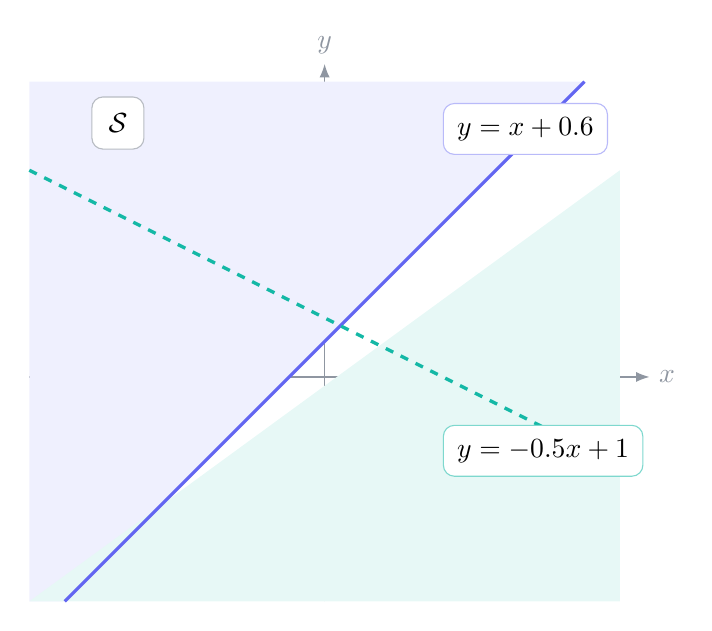
\begin{tikzpicture}[font=\sffamily,>=Latex,x=.75cm,y=.75cm]
  \draw[->,ink!55] (-5,0)--(5.5,0) node[right] {$x$};
  \draw[->,ink!55] (0,-3.8)--(0,5.3) node[above] {$y$};
  \fill[nebula!10] (-5,-3.8)--(-5,5)--(4.4,5)--(-4.4,-3.8)--cycle;
  \fill[spark!10] (-5,-3.8)--(5,-3.8)--(5,3.5)--cycle;
  \draw[very thick,nebula] (-4.4,-3.8)--(4.4,5);
  \draw[dashed,very thick,spark] (-5,3.5)--(5,-1.5);
  \node[draw=nebula!45,rounded corners=4pt,fill=white,inner sep=5pt] at (3.4,4.2) {$y=x+0.6$};
  \node[draw=spark!55,rounded corners=4pt,fill=white,inner sep=5pt] at (3.7,-1.25) {$y=-0.5x+1$};
  \node[draw=ink!35,rounded corners=4pt,fill=white,inner sep=6pt] at (-3.5,4.3) {$\mathcal S$};
\end{tikzpicture}
\end{document}
